\section{Overview}
For the last decade, the common paradigm in the use of deep learning has been to improve model performance by improving architecture and scale. These models, feature larger and larger layers that are highly interconnected, otherwise referred to as dense. While this approach has continuously led to improvements in model performance it is not without drawbacks. In 2011 a state-of-the-art computer vision model could run using a laptop. Now running a state-of-the-art language mode requires a cluster of specialized GPUs which can cost upwards of \$100,000 dollars and draw kilo-watts of power. \\
Inspired by the sparsity of the connections of neurons in the brain, unstructured sparsity seeks to improve the model efficiency by turning densely connected models into sparse models which as a result are far more efficient. While a large portion of existing research has focused on theory and high-level implementations our work is focused on using the same sparsity to realize true measurable inference speedups. 
\section{OBERT: Compressing Language Models Using Unstructured Sparsity}
\begin{figure}[!htb]
    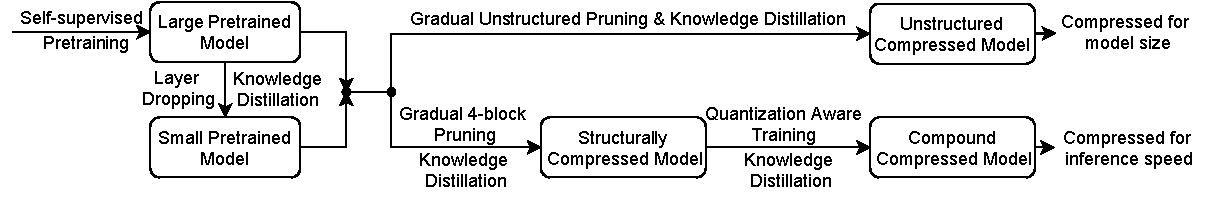
\includegraphics[scale=0.8]{media/compound-compression.pdf}
    \centering
    \caption{Overview of our compound compression approach.}
    \label{fig:compoundingsparse}
    \vspace{-1.2em}
\end{figure}
When using language models for large-scale inference there is a careful optimization process trading off model speed and accuracy. The majority of work has focused on improving model inference speed by performing structural changes which decrease the computational overhead. While approaches seeking to introduce unstructured sparsity have to be used to create models like SparseBERT \cite{Shi2021SparseBERTRT} and PruneBERT \cite{Sanh2020MovementPA}, their use of sparsity introduces large losses in accuracy. \\
\begin{figure}[!htb]
    \centering
    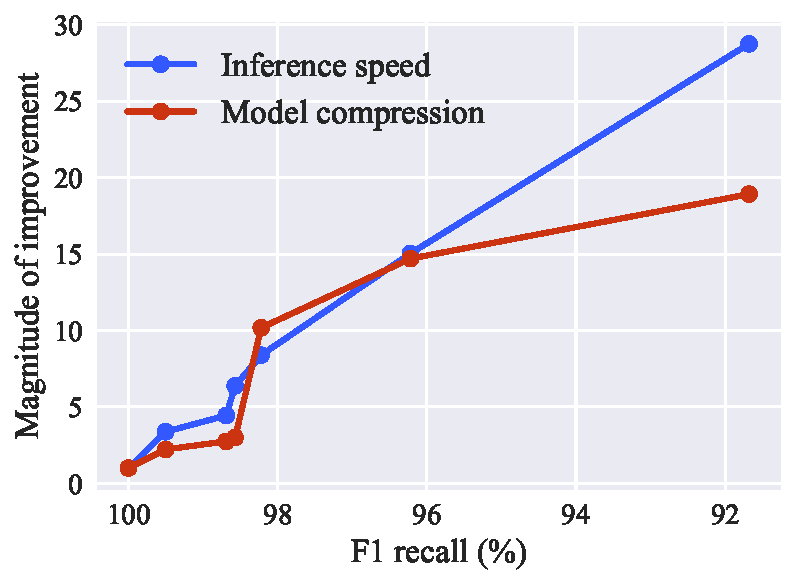
\includegraphics[scale=0.7]{media/inf_vs_comp.pdf}
    \vspace{-1em}
    \caption{F1 recall of uncompressed self-distilled 12-layer BERT-base baseline on SQuAD v1.1 relative to improvements in model inference speed and size.}
    \label{fig:inference}
\end{figure}
In this work, we introduce OBERT, which is both a sparse general-purpose language model and a framework for pruning language models of kinds. In our work, we demonstrate how second-order pruning approaches can be used to compress language models without the traditional loss in accuracy. As shown in table \ref{fig:obert-perf}, we are able to prune language models to high degrees of sparsity and extract levels of performance that were not previously considered possible.  Moreover, our approach demonstrates how well simple pruning heuristics like magnitude pruning can work as they outperform previous work by about 10\%. \\
\begin{figure}[!htb]
    \centering
    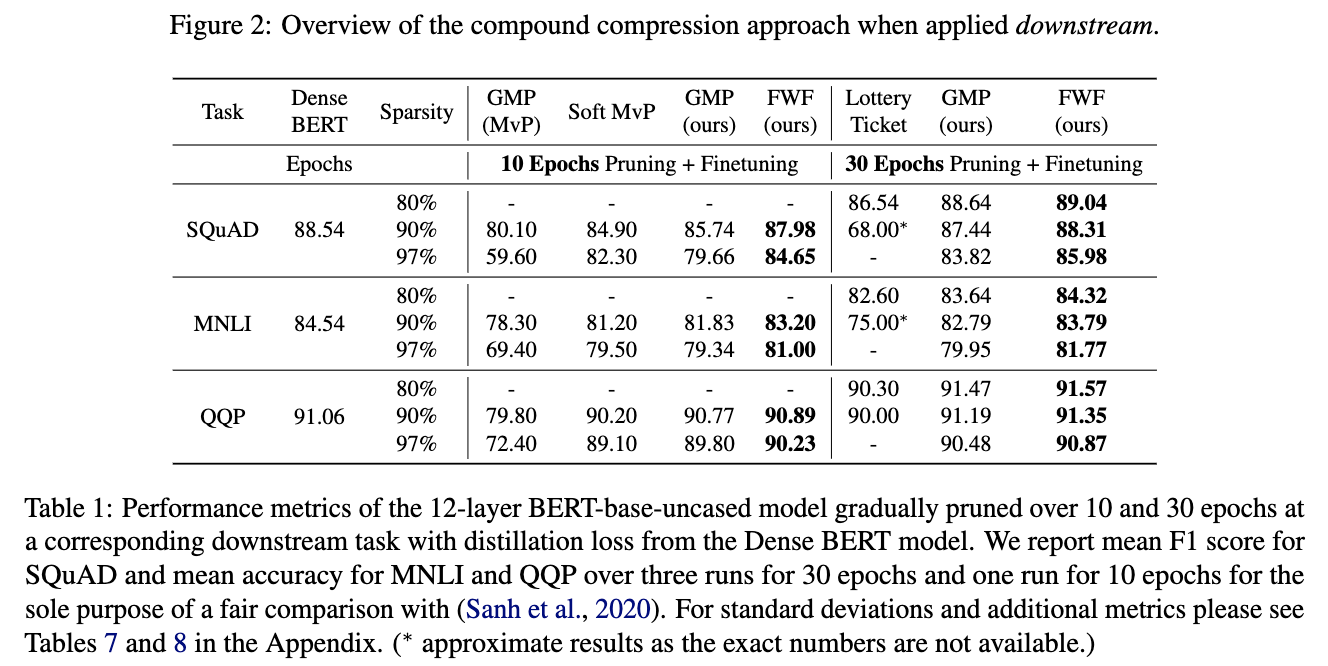
\includegraphics[scale=0.75]{media/OBERTA-Perf.png}
    \vspace{-1em}
    \label{fig:obert-perf}
\end{figure}
Leveraging second-order pruning, quantization, and knowledge distillation we formalize an approach for \textit{compounding compression} as shown in figure \ref{fig:compoundingsparse}. Each form of compression is combined and optimized to provide the highest improvements in model inference with the lowest losses in accuracy. As shown in figure \ref{inference} compounding compression can be leveraged to improve the efficiency of a system by 30x with less than 10\% loss in accuracy. 
\section{Sparse*BERT: Sparse Models Are Robust}
\begin{figure}[!htb]
    \centering
    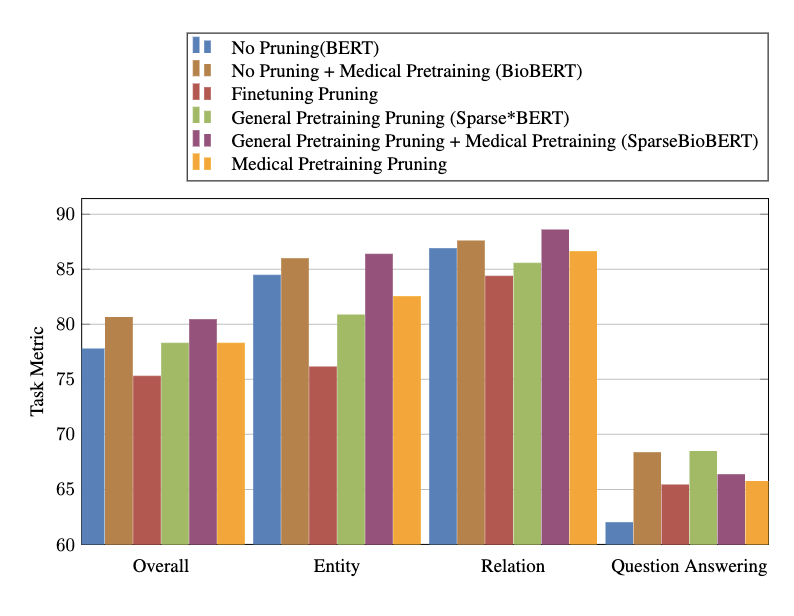
\includegraphics[scale=1.0]{media/figure1.png}
    \vspace{-1.2em}
\caption{Impact of stage and domain of pruning when evaluating BERT base uncased on medical NLP Entity Extraction, Relation Extraction, and Question Answering. For pruned and unpruned models medical pretraining can improve performance and the performance of the pruned model and the performance of BioBERT and SparseBioBERT is equivalent.}
\label{fig:sparse_transfer_categorical}
\end{figure}
Prior work on leveraging unstructured sparsity for language models has shown that taking introducing sparsity is a direct and effective way of compressing model for improved inference \cite{Zafrir2021PruneOF} \cite{Kurti2022TheOB}. Despite this work there has been little study in understanding how well sparse models can be used across tasks and domains without additional knowledge. In this work we study how sparse model can be transferred to novel tasks and domain. We explore how a sparsity can impact performance on a benchmark of 10 language understanding tasks in the domain of bio-medicine, previously unstudied in sparsity. As shown in figure \ref{fig:sparse_transfer_categorical}, we find that sparse models can be transferred to novel domains and be used without any additional optimization. Moreover, we find that models which are pruned on general domain language modeling out perform those which are pruned with domain specific language modeling or even downstream task prunning. 
\section{Future Works}
Currently, we have been working on expanding our approaches in generating sparse language models for efficiency with our proposed work: OBERTA. OBERTA builds on our prior work on leveraging unstructured sparsity for efficiency inference but is able to provide large gains in accuracy because of our use of more optimized dense language models, improved distillation and training regimes, and optimized Quantization workflows. As shown in table \ref{tab:OBERTA-squad} our OBERTA 90\% model exceeds the performance of existing sparse 24 transformers layer sparse models despite being half the size. Our OBERTA 95\% model is able to exceed the performance of existing sparse 12-layer models with 5\% higher sparsity. We will expand this work to include structurally pruned models, improved quantization, and benchmarking on a wide variety of datasets such as SQUAD v1.1 \cite{Rajpurkar2016SQuAD10} and SQUAD v2.0 \cite{Rajpurkar2018KnowWY} for question answering, QQP \footnote{https://quoradata.quora.com/First-Quora-Dataset-Release-Question-Pairs} and MNLI \cite{Williams2018ABC} for  text classification, SST-2 \cite{Socher2013RecursiveDM} for sentiment analysis, IMDB for document Classification \cite{Maas2011LearningWV}, and CONLL2003 \cite{Sang2003IntroductionTT} for token classification.
\begin{table}[!ht]
    \centering
    \begin{tabular}{|l|l|l|l|}
    \hline
        Model & Sparsity & Transformer Layers & SQUAD F1  \\ \hline
        BERT base & 0 & 12 & 88.54  \\ \hline
        BERT Large & 0 & 24 & 90.93   \\ \hline
        Prune OFA Base & 90 & 12 & 87.25  \\ \hline
        Prune OFA Large & 90 & 24 & 90.02\\ \hline
        OBERT & 90 & 12 & 88.31 \\ \hline
        OBERT & 90 & 24 & 89.96  \\ \hline
        SparseBERT & 80 & 12 & 82.5  \\ \hline
        OBERTA & 90 & 12 & 91.0 \\ \hline
        OBERTA & 95 & 12 & 89.14  \\ \hline
    \end{tabular}
    \caption{OBERTA 90\% outperforms models 2 times as large on the SQUAD v1.1 dataset.}
    \label{tab:OBERTA-squad}
\end{table}